\chapter{Trajectory Plot}
\label{appx:simulation}

\newpage
\begin{figure}[H]
	\centering
	\begin{tikzpicture}
		
		% Main trajectory image
		\node[anchor=south west, inner sep=0] (main) at (0,0)
		{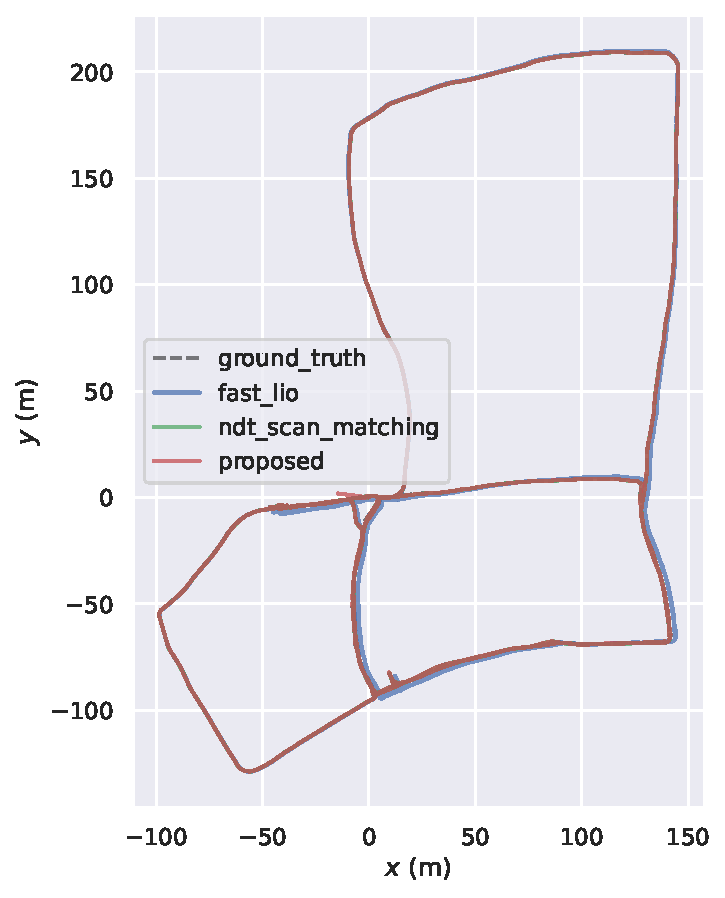
\includegraphics[width=0.9\textwidth]  {images/trajectory_plot_seq3.pdf}};
		% Coordinate system normalized to the image
		\begin{scope}[x={(main.south east)}, y={(main.north west)}]
			% Red dashed rectangle for zoom box (adjust coordinates!)
			\draw[red, thick, dashed] (0.8, 0.4) rectangle (0.95, 0.5);
			% Red arrow from zoom box to zoomed-in image
			\draw[->, red, thick] (0.8, 0.45) -- (0.45, 0.7);
		\end{scope}
		
		% Zoomed-in image overlay (use exact x/y in cm to place)
		\node[anchor=south west] at (0.2, 10.3)
		{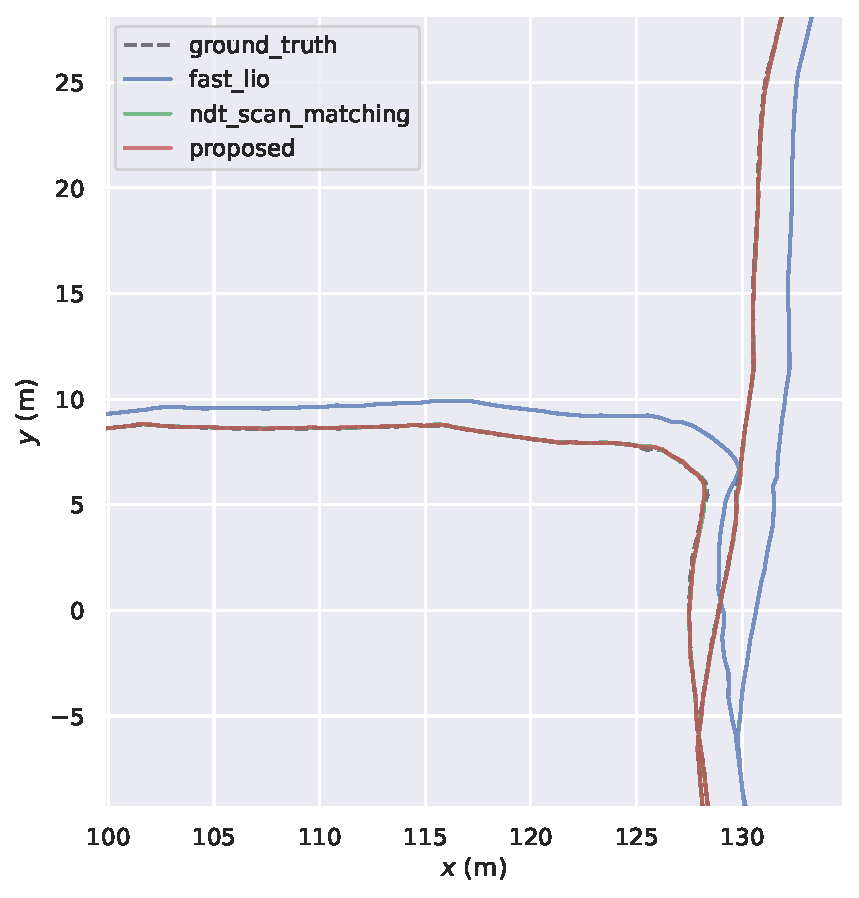
\includegraphics[width=0.37\textwidth]{images/trajectory_zoom_seq3.pdf}};
		
		% Optional label
		%\node at (15, 4.6) {\small Zoomed-in detail};
		
	\end{tikzpicture}
	
	\caption{Full trajectory with a zoomed-in view overlaid for detailed comparison. The red dashed box indicates the zoomed region.}
	\label{fig:trajectory-zoom-overlay}
\end{figure}




